\setchapterimage[2cm]{../images/header-stx.jpg}
%\setchapterpreamble[u]{\margintoc}
\chapter{Sunflower-saxitoxin complexes}
\labch{stx}

\begin{marginfigure}
    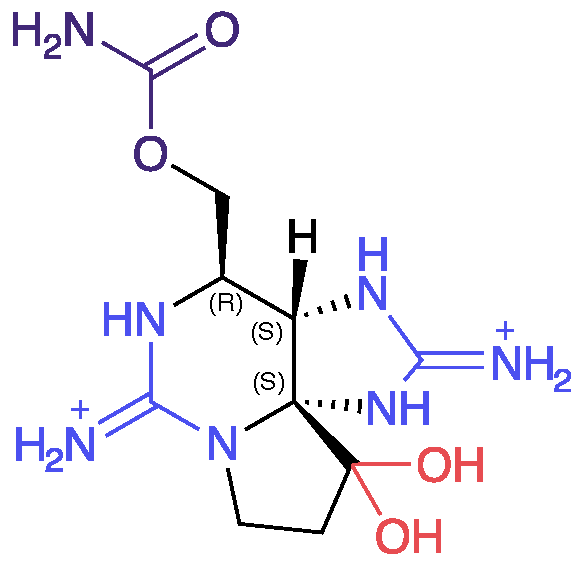
\includegraphics{stx-structure}
    \caption[Structure of STX]{Structure of STX}
    \labfig{stx-structure}
\end{marginfigure}

Having obtained a general characterization of the sunflower-type molecules and their spectroscopy, it's time to get back to the problem at hand and start looking into how they can be applied.

Let's reintroduce the molecule that motivated this whole study: saxitoxin (STX).
For the purposes of this study, the STX structure features two guanidinium moieties (which are easily susceptible to protonation), two hydroxyl, and one carbamate group as it can be seen in \reffig{stx-structure}.

The STX being doubly protonated in the figure is not an arbitrary choice.
While studying its acid-base behavior in previous work we faced a certain issue: the STX molecule has many possible protonated variations, and at the pH of real life samples, there would be a coexistence of several of them.
This was a problem, because having to apply the study to these different multiple forms in order to account for the situation would greatly increase the number of calculations.
After some thought, it was decided that the simplest way to solve this issue would be to work at a pH where only one of the protonated species would be present at a significant amount.
It was found that, at the moderate pH value of 6, the majority of the STX could be found as its doubly protonated form.
Since in real life experimental conditions attaining a pH of 6 in an hypothetical water-based sample would only imply the addition of a few drops of dilute acid, it was decided that all further studies would be carried out using such diprotonated structure.

\section{Spectroscopic study of lone STX}
The goal of this work was presented as \q{finding suitable substrate to aid in the detection of STX} from the beginning, but this desire came from a place of previous study and understanding about the spectroscopic properties of the lone STX.

This section aims to display and share the most important of these previously known facts, which are about the behavior of saxitoxin in both vibrational and electronic spectroscopy contexts.

\subsection{Vibrational spectroscopy}
As a non linear molecule with 40 atoms, STX presents a total of 114 vibrational normal modes.
\blindtext

\subsubsection{Raman spectrum}
\blindtext

\begin{figure}
    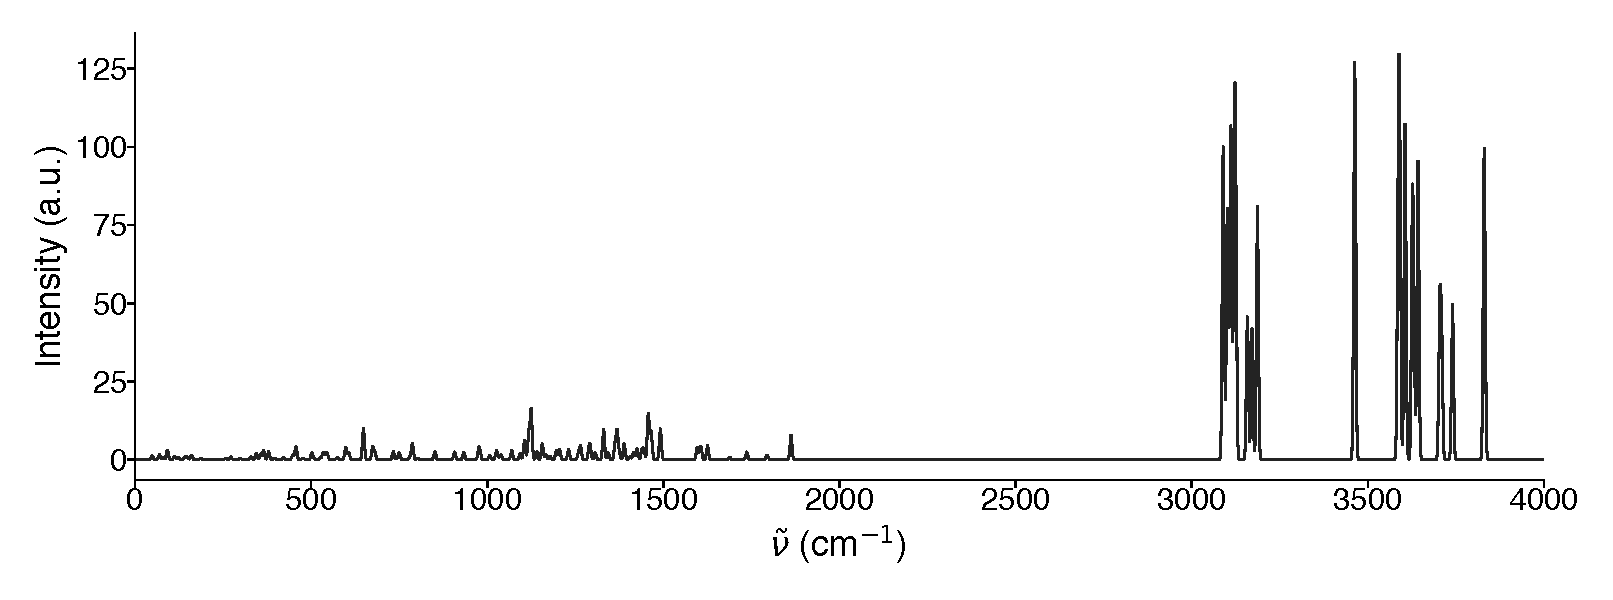
\includegraphics{raman-stx}
    \caption[Raman spectrum of lone STX]{Raman spectrum of lone STX}
    \labfig{raman-stx}
\end{figure}


\subsection{Electronic spectroscopy}
STX doesn't have any special chromophore groups, and its excited states are available at the UV range of electromagnetic radiation.
Nevertheless, it's important to identify and study this transitions in order to facilitate the application of further techniques.

\subsubsection{UV-vis spectrum}
As before, using TD-DFT as implemented in Gaussian09, the first 50 electronic transitions were calculated and used to generate the UV-vis spectrum of STX, displayed in \reffig{uv-stx}.

\begin{figure}
    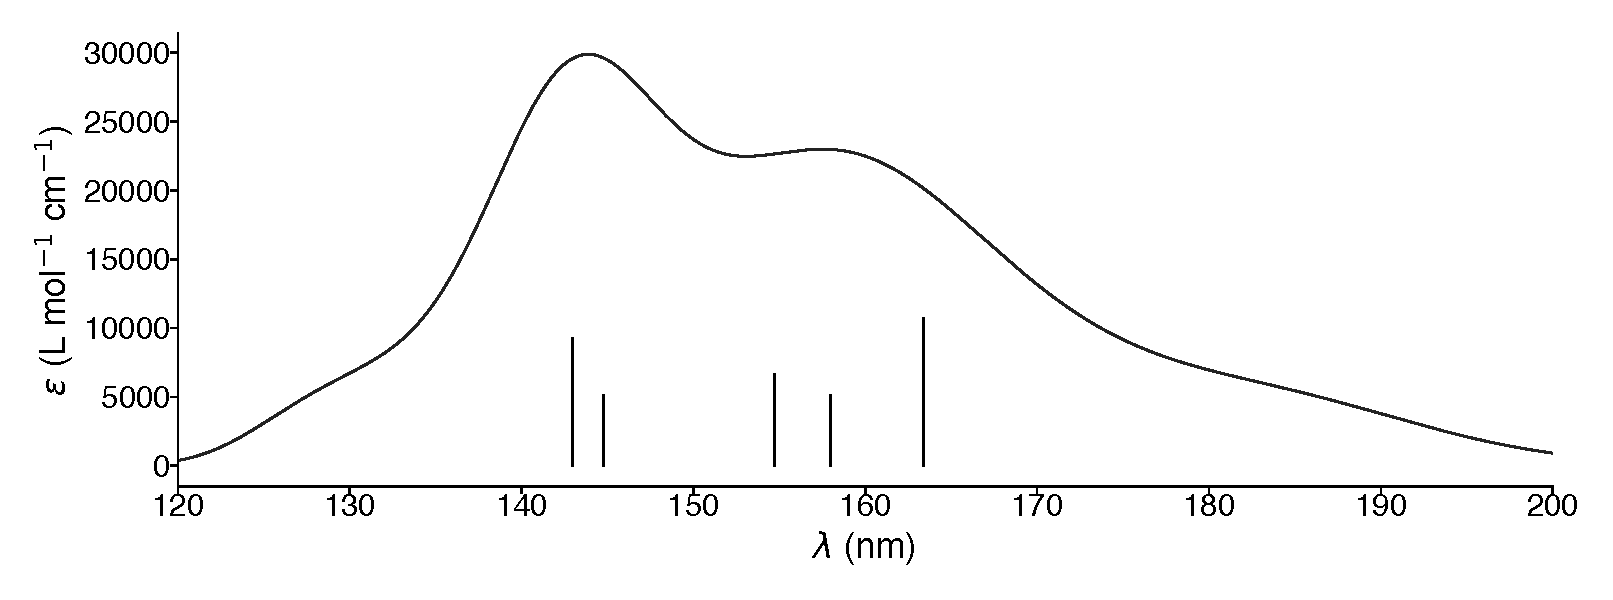
\includegraphics{uv-stx}
    \caption[UV-vis spectrum of lone STX]{UV-vis spectrum of lone STX, the 5 electronic transitions with the largest contributions have been annotated}
    \labfig{uv-stx}
\end{figure}

As it may be noted, the range of absorption (between \SI{120}{\nano\metre} and \SI{200}{\nano\metre}) is located within the UV region.
\fix{Introduce Resonance Raman here??? I'm not sure.}

\section{Study of adsorption}

After having characterized the spectroscopic profile of STX, it's time to assess its interactions with the members of the sunflower family, keeping in mind that the main goal of this work is determining if any of them could be a substrate suitable for its detection.
The first study that must be carried out, before any spectroscopic technique can be applied, is that of adsorption: how does STX adhere to the flowers, how stable is the resulting complex, what is the nature of that interaction...
This is a crucial matter, as there's no point in calculating spectra for a system that isn't stable.

\subsection{Sampling and optimization}

\begin{margintable}
    \centering
    \caption[Energies of STX-S08 conformers]{Relative energies of the STX-S08 conformers, with respect to the most stable one}
    \begin{tabular}{@{}l
                       S[table-format=2.3]@{}}
        \toprule
        System ID & {Rel. E (\si{\kilo\calorie\per\mole})} \\
        \midrule
        STX-S08-1 & 0.000 \\
        STX-S08-2 & 1.337 \\
        STX-S08-9 & 7.133 \\
        STX-S08-7 & 7.504 \\
        STX-S08-6 & 9.896 \\
        STX-S08-4 & 18.554 \\
        STX-S08-3 & 20.321 \\
        STX-S08-10 & 21.734 \\
        STX-S08-5 & 22.529 \\
        STX-S08-8 & 29.715 \\
    \end{tabular}
    \labtab{stx-s08-energies}
\end{margintable}

In order to take into account the possible conformational variability, the STX was manually given an array of different relative positions and angles with respect to the surface of the flowers.
Following this idea, 10 different variations were modeled for each of the 18 STX-sunflower pairs, resulting in a total of 180 structures.
These various orientations will be referred to as \q{conformers}.
All of the conformers for each pairing were optimized at the M06-2X/def2SVP calculation level, and their final energies were compared in order to identify the most stable ones and discard the unstable.
Taking the STX-S08 system as an example, the relative energies of all of its generated conformers are displayed in \reftab{stx-s08-energies}.
As it can be seen, the most stable conformer (MSC) is STX-S08-1.
However, STX-S08-2, STX-S08-9 and STX-S08-7 are also close energy-wise.
A question arises, how can we determine which conformers are stable enough to be important, and which are not?

\begin{figure}
    \includegraphics{s08-conformers}
    \caption[Conformers of STX-S08]{Examples of conformers of the STX-S08 system, from left to right, STX-S08-1, STX-S08-9, and STX-S08-3}
    \labfig{s08-conformers}
\end{figure}

\begin{margintable}
    \centering
    \caption[Maxwell-Boltzmann populations of STX-S08]{Maxwell-Boltzmann populations of the STX-S08 conformer set, expressed as percentages}
    \begin{tabular}{@{}l
                       S[table-format=2.2]@{}}
        \toprule
        System ID & {Population (\si{\percent})} \\
        \midrule
        STX-S08-1 & 58.56 \\
        STX-S08-2 & 34.16 \\
        STX-S08-9 & 3.30 \\
        STX-S08-7 & 2.83 \\
        STX-S08-6 & 1.08 \\
        STX-S08-4 & 0.03 \\
        STX-S08-3 & 0.02 \\
        STX-S08-10 & 0.01 \\
        STX-S08-5 & 0.01 \\
        STX-S08-8 & 0.00 \\
    \end{tabular}
    \labtab{stx-s08-populations}
\end{margintable}

\subsection{Maxwell-Boltzmann statistics}
Our answer to this problem consisted in applying Maxwell-Boltzmann statistics to transform these energies into population fractions.
This concept essentially translates as the fraction of each conformer that would be present in a macroscopic sample at a certain temperature.
As modeled in \refeq{maxwell-boltzmann}, $p_i$ represents the population fraction of the conformer $i$, while $p_\textit{MSC}$ is the fraction of the MSC of that particular set of conformers.
As for the rest of the elements of the equation, $\varepsilon$ corresponds to the absolute energies of the systems, $N$ is the total number of conformers in each set (which is 10 in our case), $k$ is Boltzmann's constant, and $T$ is the temperature of the system in \si{\kelvin} (which for the purposes of this study is set at \fix{\SI{298}{\kelvin}, or is it 273??}).

\begin{align}
\begin{split}
    \labeq{maxwell-boltzmann}
    \frac{p_i}{p_\textit{MSC}}&=e^{\varepsilon_\textit{MSC}-\varepsilon_i/kT} \\
    \sum_{i=1}^{N}\frac{p_i}{p_\textit{MSC}}&=\frac{\sum_{i=1}^{N}p_i}{p_\textit{MSC}}=\frac{1}{p_\textit{MSC}} \\
    \frac{p_i/p_\textit{MSC}}{1/p_\textit{MSC}}&=\frac{e^{\varepsilon_\textit{MSC}-\varepsilon_i/kT}}{\sum_{i=1}^{N}\frac{p_i}{p_\textit{MSC}}}=p_i \\
\end{split}
\end{align}

Continuing with the example, the populations for STX-S08 were computed and are displayed in \reftab{stx-s08-populations}.
As an arbitrary threshold, it was decided to filter out all of the conformers with populations lower than \SI{1}{\percent}, and to just keep studying the remaining ones.
That is, all further calculations that involve the computation of weighted mean values or spectra will only take into account conformers with populations higher than that value.

\begin{table}
    \centering
    \caption[Maxwell-Boltzmann populations for all sets]{Maxwell-Boltzmann populations for the 5 most stable conformers in all sets, as percentages, with non significant conformers marked in grey}
    \begin{tabular}{@{}c
                    S[table-format=2.2]
                    S[table-format=2.2]
                    S[table-format=2.2]
                    S[table-format=2.2]
                    S[table-format=2.2]
                    S[table-format=2.2]@{}}
        \toprule
        System & {S} & {Se} & {As} & {AsN} & {P} & {PN} \\
        n of petals & {\si{\percent}} & {\si{\percent}} & {\si{\percent}} & {\si{\percent}} & {\si{\percent}} & {\si{\percent}} \\
        \midrule
        \multirow{5}{*}{08}
        & 58.56 & 79.24 & 60.96 & 81.32 & 40.79 & 65.13 \\
        & 34.16 & 15.57 & 35.22 & 15.98 & 37.48 & 29.71 \\
        & 03.30 &  1.90 &  2.19 &  2.16 & 20.53 &  4.61 \\
        &  2.84 &  1.15 &  1.38 &  \color{fd}0.25 &  \color{fd}0.44 &  \color{fd}0.24 \\
        &  1.08 &  \color{fd}0.14 &  \color{fd}0.16 &  \color{fd}0.23 &  \color{fd}0.32 &  \color{fd}0.21 \\
        \\
        \multirow{5}{*}{10}
        & 38.68 & 61.74 & 99.64 & 100.00 & 86.97 & 51.05 \\
        & 36.07 & 38.26 &  \color{fd}0.30 &   \color{fd}0.00 & 10.12 & 46.11 \\
        & 25.21 &  \color{fd}0.00 &  \color{fd}0.00 &   \color{fd}0.00 &  2.83 &  2.26 \\
        &  \color{fd}0.02 &  \color{fd}0.00 &  \color{fd}0.00 &   \color{fd}0.00 &  \color{fd}0.06 &  \color{fd}0.56 \\
        &  \color{fd}0.01 &  \color{fd}0.00 &  \color{fd}0.00 &   \color{fd}0.00 &  \color{fd}0.02 &  \color{fd}0.01 \\
        \\
        \multirow{5}{*}{12}
        & 99.99 & 58.93 & 99.75 & 97.75 & 93.29 & 93.83 \\
        &  \color{fd}0.01 & 18.98 &  \color{fd}0.10 &  2.23 &  3.26 &  5.97 \\
        &  \color{fd}0.00 & 14.52 &  \color{fd}0.08 &  \color{fd}0.01 &  2.42 &  \color{fd}0.20 \\
        &  \color{fd}0.00 &  6.03 &  \color{fd}0.04 &  \color{fd}0.00 &  \color{fd}0.74 &  \color{fd}0.00 \\
        &  \color{fd}0.00 &  1.55 &  \color{fd}0.02 &  \color{fd}0.00 &  \color{fd}0.16 &  \color{fd}0.00 \\
        \bottomrule
    \end{tabular}
    \labtab{maxwell-boltzmann-all}
\end{table}

\subsection{Basis Set Superposition Error correction}
These optimization calculations have served as a way to estimate the populations of the conformers and to identify the most stable and relevant ones.
However, they cannot be used directly to obtain accurate values for the interaction energies due to the Basis Set Superposition Error (BSSE).
In this case, this error arises when the STX molecule is close to the sunflower and their basis functions overlap.
The part of STX basis functions that comes near the sunflower improves its part of the calculation, and vice versa.
This is a problem because in order to get the interaction energy we have to subtract the energy of the complex from the energies of the isolated molecules,\marginnote{
    \begin{equation}\labeq{interaction-energy}
        V_\textit{STX-flower} = E_\textit{STX-flower} - E_\textit{STX} - E_\textit{flower}
    \end{equation}
} but the former has a better calculation level than the latter.

To solve this problem, we used the counterpoise method.
For hypothetical molecules A and B, this technique estimates their BSSE by placing the basis functions of molecule A next to molecule B, right where molecule A would go in the optimized geometry of the complex.\sidecite{duijneveldt94,rosch03}
However, its nuclei are ommited, and just the energy of A is calculated using such an extended basis set.
The same process is applied to get the corrected energy of isolated B.
Finally, the same formula as in \refeq{interaction-energy} is applied to the new values, which results in the counterpoise corrected (CC) interaction energy.

All such energies were calculated for all of the STX-flower system conformers.
Their weighted averages using the population values of \reftab{maxwell-boltzmann-all} were computed, and are displayed in \reffig{counterpoise-energies}.

\begin{figure}
    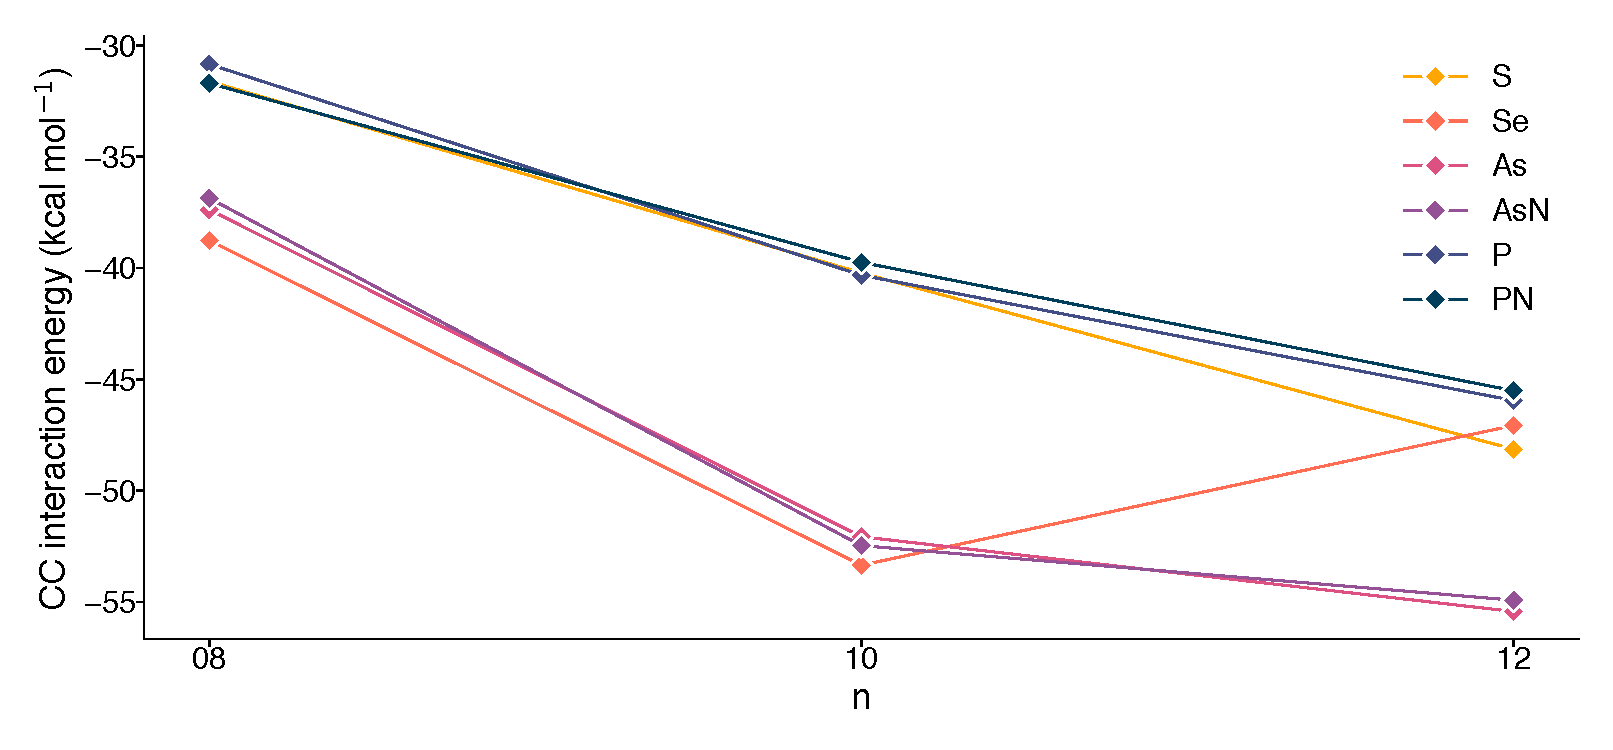
\includegraphics{counterpoise-energies}
    \caption[Counterpoise corrected interaction energies]{Counterpoise corrected interaction energies as weighted averages for all of the sets}
    \labfig{counterpoise-energies}
\end{figure}

As it can be noted, all of the systems present negative interactions energies, that is, the complex has a lower energy than the sum of the energies of its constituents.
This is a good indication that the systems are all stable and can be further studied.
All of the families (except for Se) appear to have a common tendency: the higher the amount of petals, the higher the stabilization. This could be due to the flower having a larger area and bending in a way that maximizes the interactions with the STX molecule.

\section{Study of non-covalent interactions}
\blindtext

\section{Study of UV-vis behavior}
One of the main points of adsorbing the STX to the flowers is the desire of increasing its range of absorption of UV-vis radiation.
It's possible that the flower-STX complex absorbs light at longer wavelengths than the isolated STX, and this could be highly beneficial to apply further detection techniques based on resonace.

\subsection{General UV-vis spectroscopy}
Electronic spectra were calculated as described in \refsec{electronic-transition-study} and \refsec{spectra-envelope-calculation} for the most stable conformers of all of the sunflower-STX complexes.

First, they were plotted together with the UV-vis spectrum of STX and of their corresponding isolated flower.
The individual transitions with significant weights were also plotted as straight vertical lines.
This allowed us to compare the absorption ranges of the complex versus those of the isolated STX and flowers, and to judge if the shifting effect is good enough.

As an example of this, the UV-vis spectra of STX, S08 and S08-STX are displayed in \reffig{uv-s08}.

\begin{figure}
    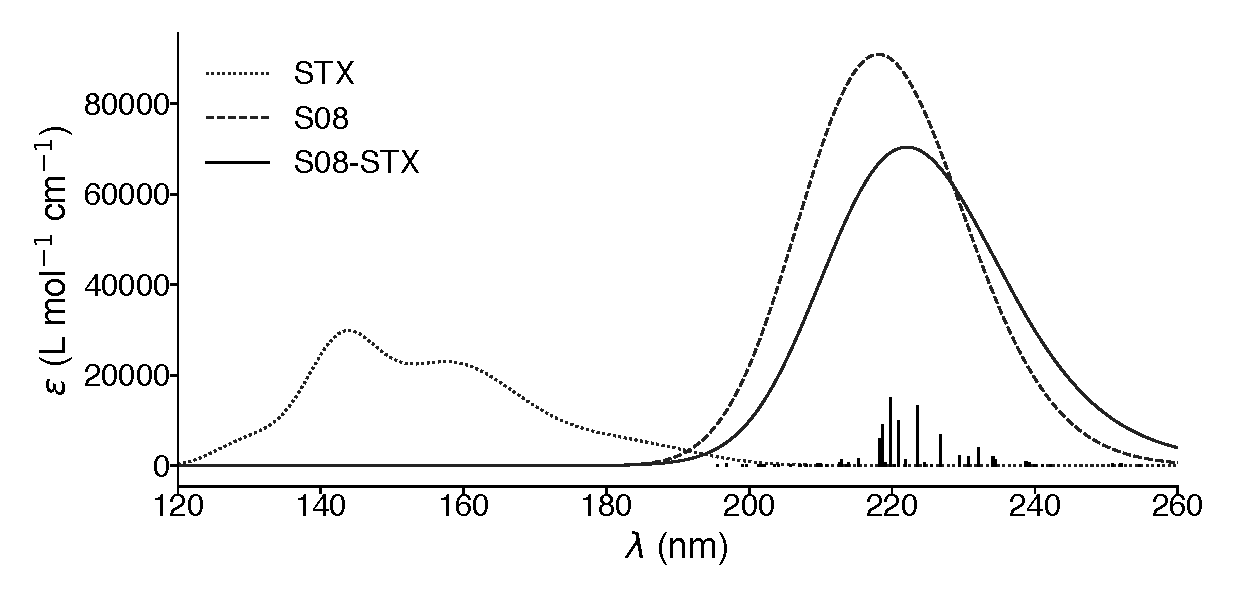
\includegraphics{uv-s08}
    \caption[UV-vis spectrum of S08-STX]{UV-vis spectra of S08-STX and its components}
    \labfig{uv-s08}
\end{figure}

As it may be noted, the spectra of the complex has almost the same absorption range as that of the isolated S08, and in any case, it's definitely shifted towards longer wavelengths in contrast with that of STX.
This effect was the same for all of the flower-STX complexes, and the full list of compared UV-vis spectra can be found in \refsec{ap:uv-vis-flowers}.

After this, the UV-vis absorption spectra of all of the complexes were plotted together in order to visually compare just their absorption ranges. This plot is displayed in \reffig{complex-uv}.

\begin{figure*}
    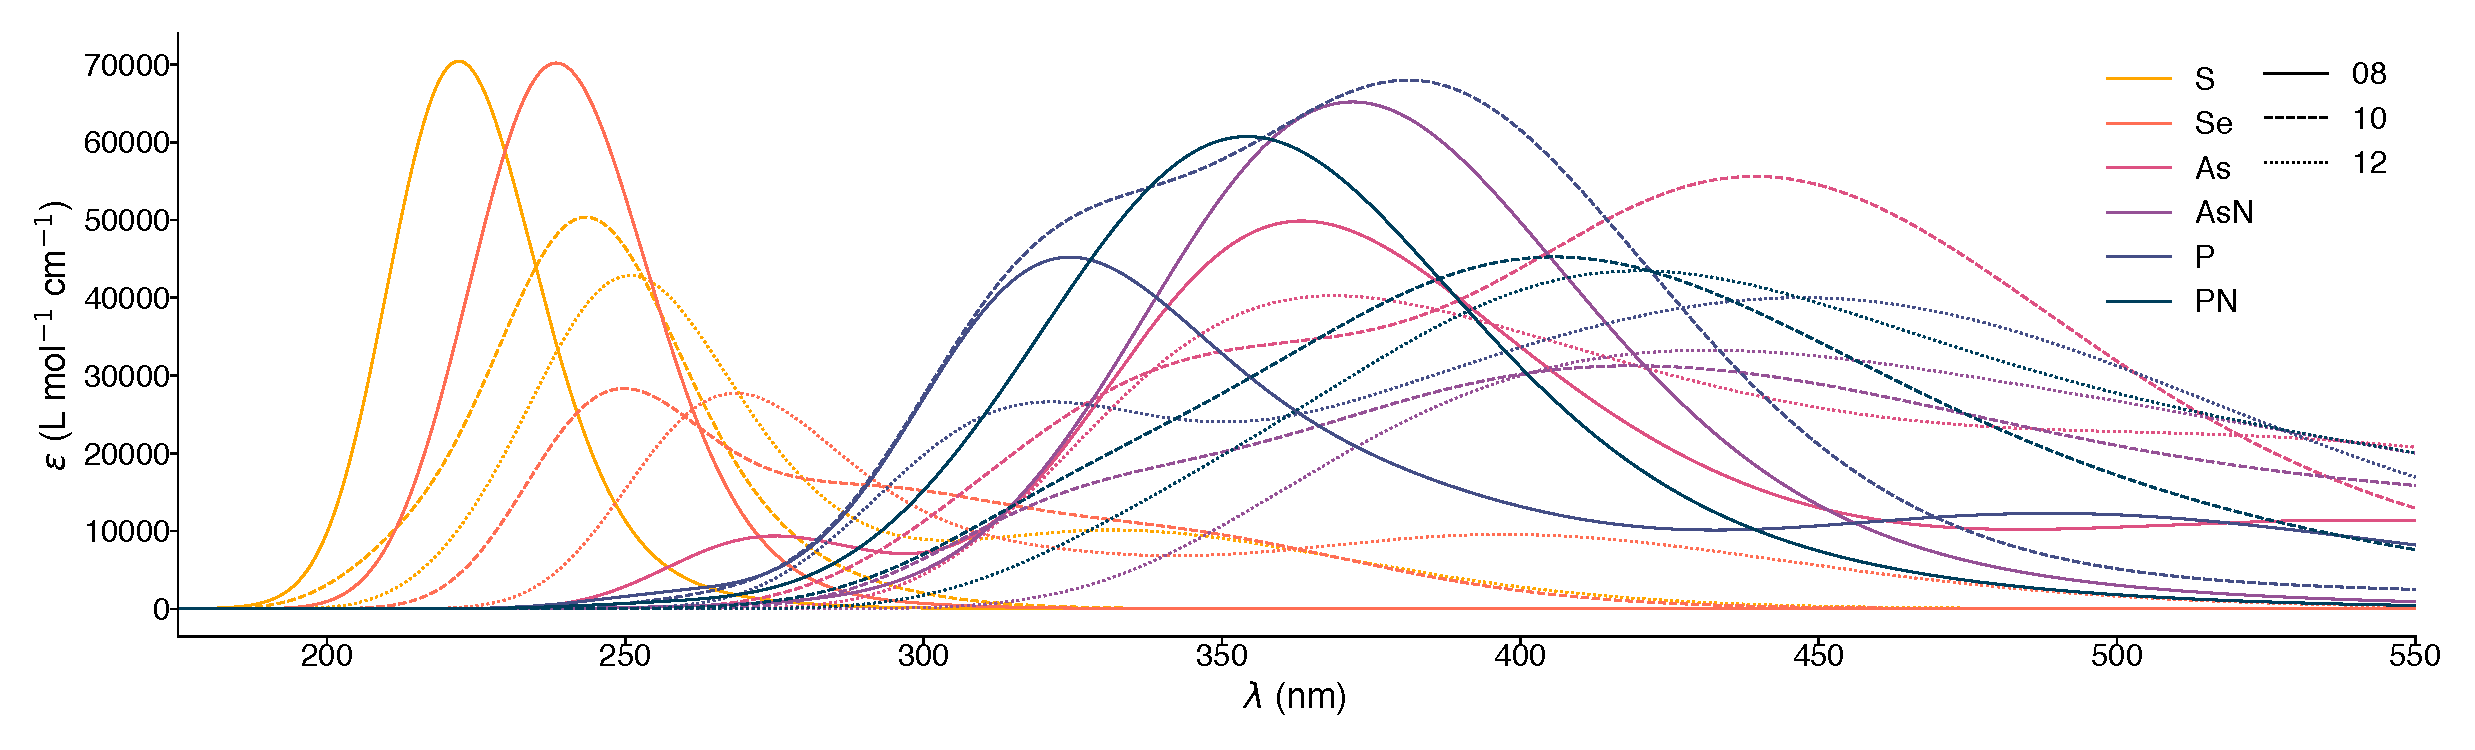
\includegraphics{complex-uv}
    \caption[UV-vis absorption spectra of all complexes]{UV-vis absorption spectra of all flower-STX complexes}
    \labfig{complex-uv}
\end{figure*}

Since this work aims to propose realistic detection techniques, it's important that the systems are actually detectable and identifiable in a real setting.
With this purpose in mind, and keeping into account the usual wavelengths of commercially available lasers for Raman,\sidenote{Which is between \fix{\SI{300}{\nano\metre} and \SI{800}{\nano\metre}}} all of the complexes with absorption ranges starting below \SI{250}{\nano\metre} were filtered out.
From the remaining ones, a select few were hand-picked according to the upper limit of their ranges and to their specific individual electronic transitions.
This left us with 8 systems out of the starting 18, which was deemed as a sufficient amount to continue with the last part of the study.

\begin{margintable}
    \centering
    \caption[UV absorption range of selected complexes]{UV absorption range of selected complexes}
    \begin{tabular}{@{}rc@{}}
        \toprule
        System & $\lambda$ (\si{\nano\metre}) \\
        \midrule
        As10 & 300-600 \\
        As12 & 300-900 \\
        AsN08 & 300-450 \\
        AsN10 & 300-650 \\
        AsN12 & 350-850 \\
        P12 & 300-700 \\
        PN10 & 300-550 \\
        PN12 & 325-625 \\
    \end{tabular}
    \labtab{uv-ranges}
\end{margintable}

The UV absorption range for those remaining complexes was also displayed on \reftab{uv-ranges} for convenience.
\blindtext

\subsection{Charge transfer analysis}
\blindtext

\section{Resonance Raman}
At last, it was time to apply the previous parts of the study and test the performance of the selected sunflowers.
\fix{A nicer explanation of Resonance raman here? Move the one from Methods? I'm not sure...}
\blindtext
RR spectra were generated for each of the flower-STX systems by using incident laser wavelengths in their particular ranges of absorption.
Specifically, the whole of their absorption interval was covered by selecting wavelengths with a step of \SI{3}{\nano\metre}.\sidenote{So in the case of As10, for example, the Resonance raman calculations were performed with lasers of \num{300}, \num{303}, \num{306}... all up until \SI{600}{\nano\metre}}
\blindtext

\subsection{Generation and comparison of spectra}
\labsec{heatmaps}
The RR calculations from the previous step amounted to a total of 2858, where the amplification, position and relevance of each vibrational mode\sidenote{Between \num{186} and \num{222} depending on the size of the flower} had to be evaluated.
For this purpose, the two following metrics were developed.

\subsubsection{Individual molecule contribution to a complex vibrational mode}
The first of these evaluations was differentiating which vibrational normal modes involve the vibration of the flower, which modes involve the vibration of the STX, and which modes are mixed.
As introduced in \refsec{intmodes-methods}, this was done by analyzing the displacements of the vibrations translated into redundant internal coordinates.
To understand how this is done, we will use the As12-STX system as an example.
The standard Gaussian09 output describes normal modes as cartesian displacements of normal coordinates, indicating vectors for each atom.
For instance, the beginning of the output of vibrational normal mode number 42 looks like this:

\begin{lstlisting}[label=normal-mode-output, style=kaolstplain]
                    42
                     A
Frequencies --    229.2846
Red. masses --     36.2305
Frc consts  --      1.1222
IR Inten    --      3.9161
Atom  AN      X      Y      Z
   1  33    -0.15  -0.08   0.01
   2  33    -0.03  -0.04  -0.04
   3   6     0.13   0.06   0.06
   4   6     0.06   0.05   0.01
   5  33     0.10  -0.01  -0.03
               ...
\end{lstlisting}

This contains all of the necessary information to study the movements of the atoms and understand the vibrations of the mode, but it's difficult to interpret.
By specifying the keyword \code{intmodes} in the frequency calculation, this output gets translated into the much more readable redundant internal coordinates notation.
This is As12-STX's mode number 42 in this new format.

\begin{lstlisting}[label=intmodes-output, style=kaolstplain]
              ----------------------------
              ! Normal Mode    42        !
--------------                            --------------
! Name  Definition       Value     Relative Weight (%) !
--------------------------------------------------------
! R1    R(1,34)         -0.0693             0.4        !
! R9    R(4,63)         -0.067              0.4        !
! R15   R(8,9)           0.1332             0.8        !
! A4    A(2,3,30)       -0.0755             0.4        !
! A19   A(10,7,63)       0.0567             0.3        !
! A21   A(5,9,8)         0.1548             0.9        !
! D1    D(36,1,34,24)    0.0965             0.5        !
! D3    D(34,1,36,27)    0.1767             1.0        !
! D5    D(6,2,3,4)      -0.0882             0.5        !
                          ...
\end{lstlisting}

\begin{margintable}
    \centering
    \caption[Classification of individual vibrations]{Classification of the individual vibrations of normal mode 42 for As12-STX (atoms of the flower and the STX are marked in blue and red, respectively)}
    \begin{tabular}{@{}ll@{}}
        \toprule
        Vib. def. &  Category \\
        \midrule
        R(\stx{1},\stx{34})                     & STX \\
        R(\stx{4},\flower{63})                  & Mixed \\
        R(\stx{8},\stx{9})                      & STX \\
        A(\stx{2},\stx{3},\stx{30})             & STX \\
        A(\stx{10},\stx{7},\flower{63})         & Mixed \\
        A(\stx{5},\stx{9},\stx{8})              & STX \\
        D(\stx{36},\stx{1},\stx{34},\stx{24})   & STX \\
        D(\stx{34},\stx{1},\stx{36},\stx{27})   & STX \\
        D(\stx{6},\stx{2},\stx{3},\stx{4})      & STX \\
    \end{tabular}
    \labtab{intmodes-classification}
\end{margintable}

Here the displacements are expressed as bond length extensions between two atoms (R), angle openings and closings between three (A), and dihedral angle torsions between four (D).
Their magnitude is expressed as a single positive or negative value, whose absolute value is then weighted and displayed as the Relative Weight as a percent.
By differentiating whether the atoms involved in a certain vibrational motion belong to the As12 flower or to the STX, said vibration can be classified as an exclusive flower vibration, as an exclusive STX vibration, or as a mixed one.
Such classification, illustrated in \reftab{intmodes-classification}, can be easily automated using a script.

By adding up the relative weights of the vibrations in each category, we can find out which of the elements of the flower-STX complex dominate a particular mode.
In this case, mode 42 has a \SI{92.54}{\percent} contribution from the STX, a \SI{0.00}{\percent} contribution from the flower, and a \SI{7.45}{\percent} contribution from mixed vibrations.

From a practical point of view, the fact that it's composed almost exclusively of isolated STX vibrations makes this a good choice of vibrational mode to look for in a RR spectra of this complex.
In contrast to other mixed or flower-exclusive vibrational modes, a mode like this is a clear sign of the presence of the STX.

\subsubsection{Resonance Raman enhancement factor}
Even if a mode is exclusive to our molecule of interest, it needs to have a sufficient intensity in the final spectrum: otherwise it cannot be detected and cannot be of any use in the identification.
In the context of RR, this means that it has to benefit from a certain level of amplification during resonance experiments.

To evaluate this for all of the tested laser wavelengths, the enhancement factor (EF) metric was designed and applied.
The EF for a certain vibrational mode $i$ and laser wavelength $\lambda$  is defined in \refeq{enhancement-factor}.

\begin{equation}
    \labeq{enhancement-factor}
    EF_{i,\lambda} = \log_{10}\left(\frac{I_{i,\lambda}}{I_{i,\textit{SL}}}\right)
\end{equation}

In this equation, $I_{i,\lambda}$ corresponds to the Raman activity of the mode $i$ in the amplified spectrum, and $I_{i,\textit{SL}}$ is the activity of the same mode in a regular Raman prediction.
Using a logarithmic scale makes easier to visualize the very high amplifications that arise with this technique, which in the case of this work, have reached values near \num{10e10} times than the standard Raman.

Similarly as before, this calculation is easy to automate and can serve as a way to filter out wavelengths that don't generate sufficient amplification, or discard modes that aren't sufficiently amplified.

\subsubsection{Combined resonance graphs}
In order to make use of the two newly defined metrics, an output file processing pipeline was designed.
Large amounts of data from the internal mode decompositions, standard Raman spectra and many amplified RR spectra were processed, combined and analyzed using Python scripts.

This information was filtered and displayed in the following manner:
First, Gaussian envelopes for all of the RR spectra as well as the standard Raman spectrum were calculated.
These envelopes were equivalent to those used in previous Raman spectra: 10000 points divided across the most relevant range for each system.
Then, each of the points in the amplified RR curves was converted into EF values using \refeq{enhancement-factor}.
These were plotted as a colored grid: all of the RR wavelengths on the vertical axis, and the 10000 calculated wave number values on the horizontal axis.
The squares of the grid, therefore, were colored according to the calculated EF values.

This resulted in quite colorful graphs where the brightest horizontal lines correspond to the laser wavelengths that generate larger amplifications, and bright vertical areas correspond to highly amplified vibrational modes.

Then, in order to make full use of the metrics, these graphs were annotated using a special procedure.
In regard to the vibrational modes, two thresholds were set: a maximum percent of flower contribution, and a minimum percent of STX contribution.
This ensured that the displayed modes were relevant.
As for the laser wavelengths, only the ones that produced amplifications above a certain threshold value for the EF of the previously selected vibrational modes were displayed.

Applying this method to the running example of As12-STX, then, resulted in \reffig{comb-as12}

\begin{figure}
    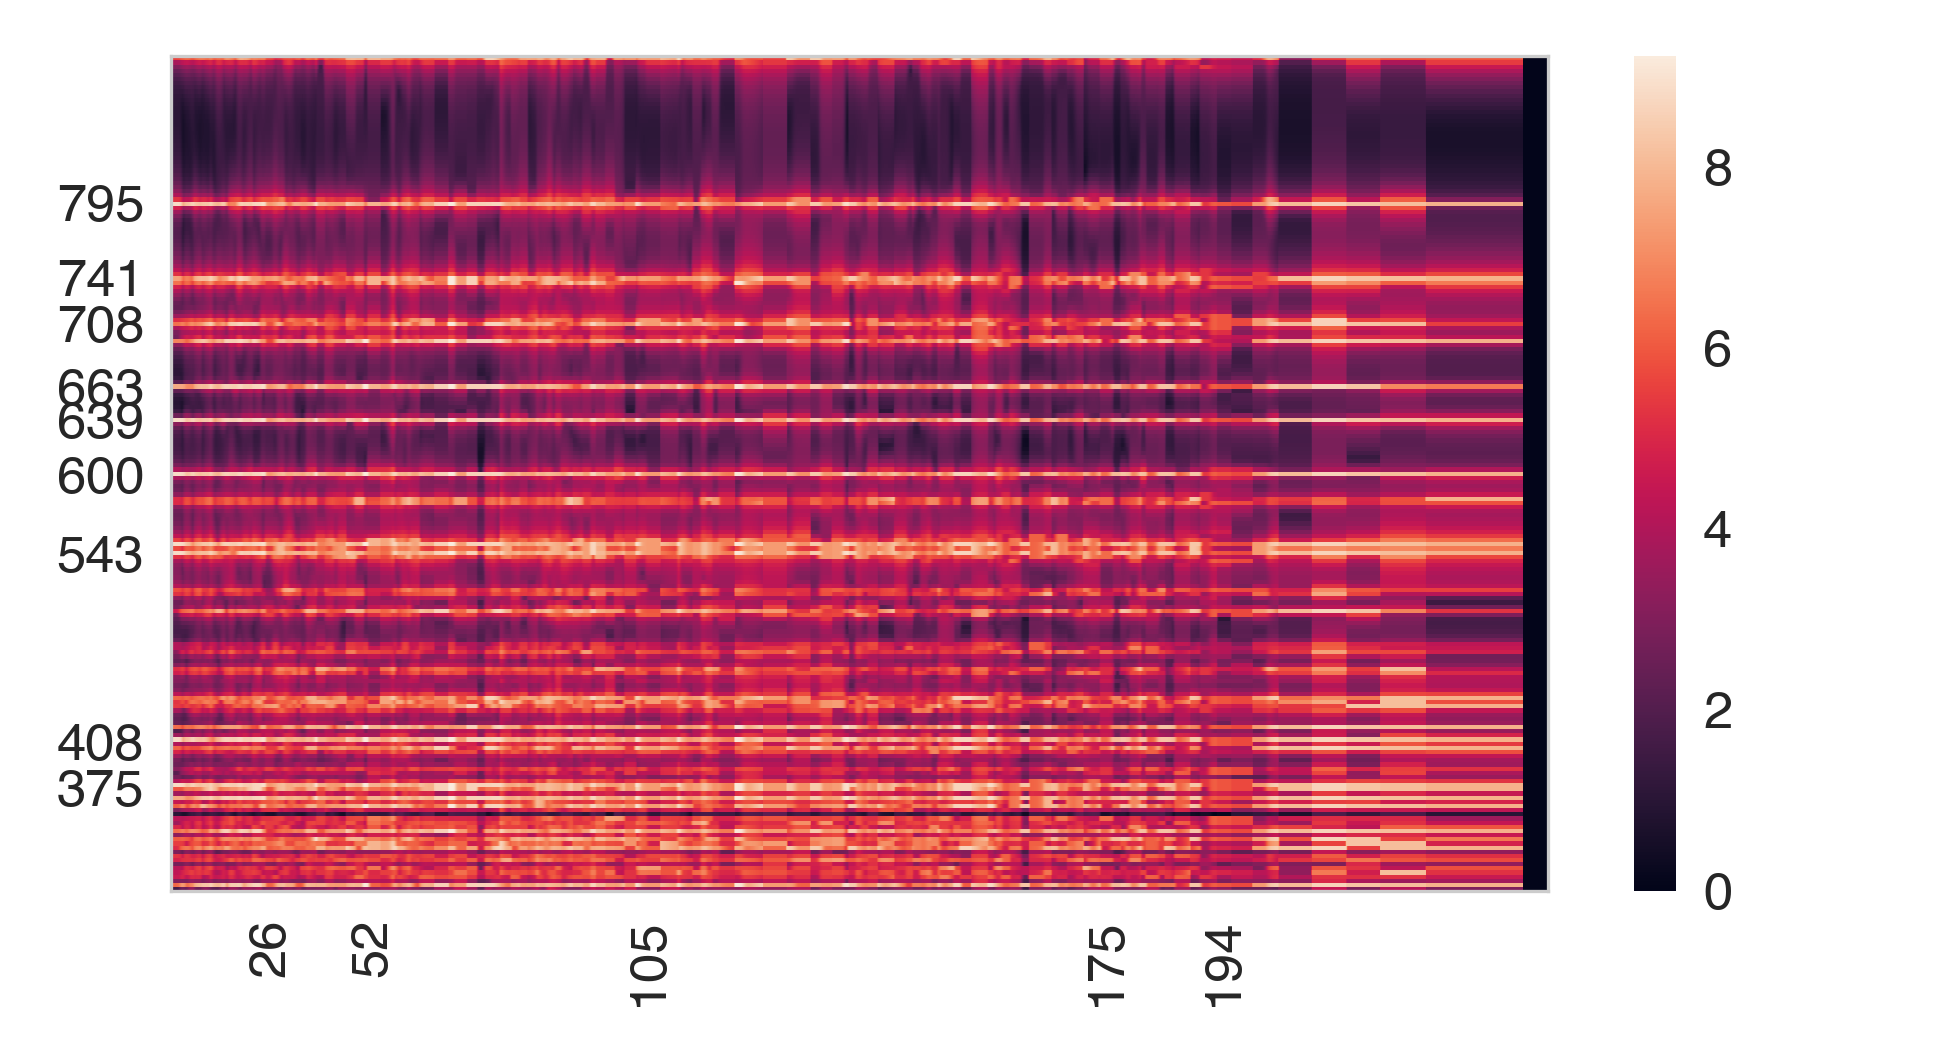
\includegraphics{comb-as12}
    \caption[Combined resonance graph for As12-STX]{Combined resonance graph for As12-STX}
    \labfig{comb-as12}
\end{figure}



\subsection{Final selection}
While the previous method serves as a convenient way to visualize the best amplifications, it's true that it deviates a little from the usual representations of Raman data.
This final section aims to tie its insights together, and displaying them in a more standard way in order to facilitate the comparison and selection of a definitive combination of flower, laser wavelength and set of vibrational modes.

For this reason, a complementary way of plotting amplified Raman spectra was designed.
